Introduction and motivation with 8 TeV cross section and rate

\begin{figure}[!h]
  \centering
  \begin{tabular}{c}
                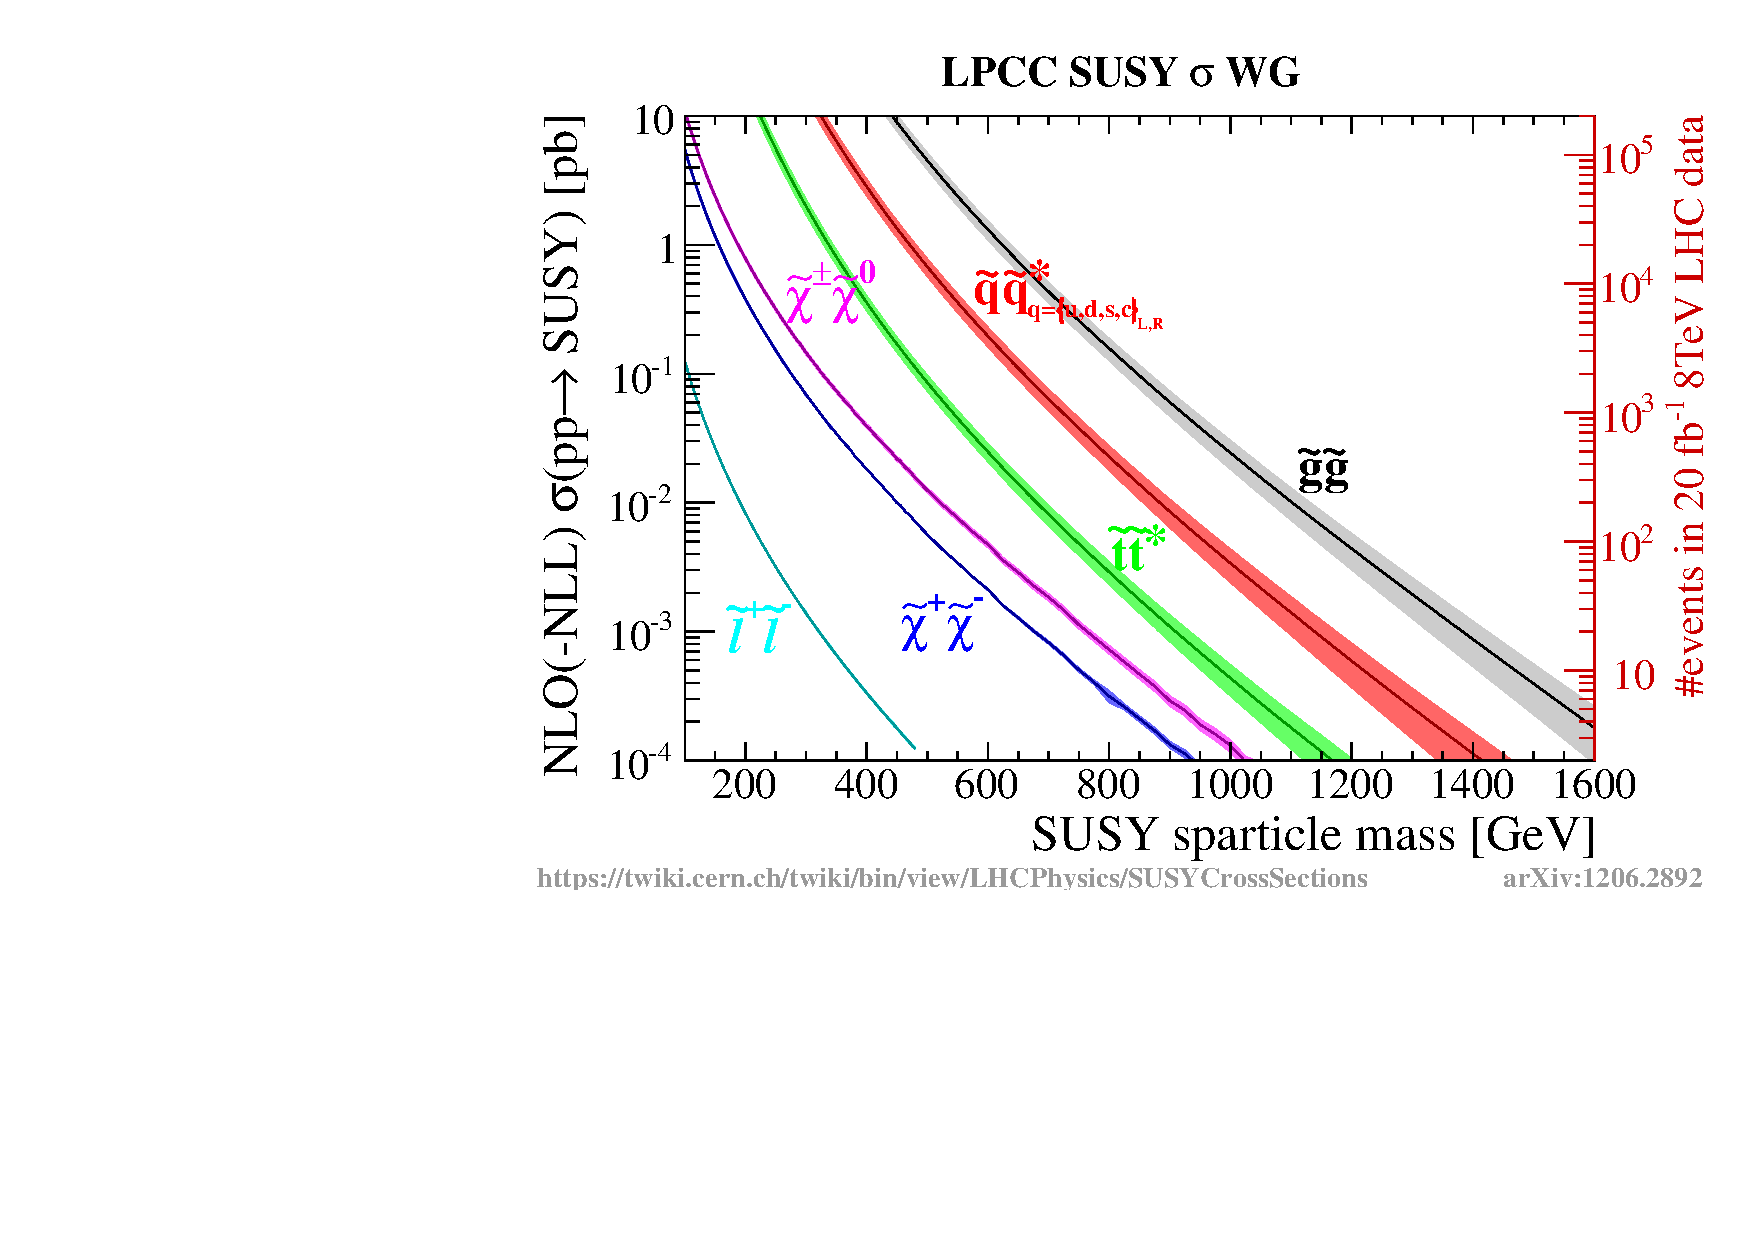
\includegraphics[width=0.65\textwidth]{figures/xsections_strong.pdf} 
  \end{tabular}
  \caption{Theory cross sections for selected SUSY processes as function of the SUSY sparticle mass. The y-axis on the right indicates the expected number of events in 20\fbinv of pp collision data at the LHC at $\sqrt{s}=8$\tev. Taken from~\cite{Kramer:2012bx}.}
  \label{fig:result_comparison}
\end{figure}

Parts of this Chapter are taken from~\cite{bib:AN-12-350}, having been written by the author. The analysis is published in~\cite{Chatrchyan:2014lfa}.  

\section{Event Selection}
\label{sec:RA2_sel}

\subsection{Data samples and trigger}
\label{subsec:RA2_samples_trigger}

\subsection{Event Cleaning}
\label{subsec:RA2_cleaning}

\subsection{Baseline Selection}
\label{subsec:RA2_baseline}

\subsection{Exclusive Search Regions}
\label{subsec:RA2_search_regions}

\section{QCD Background Estimation with the Rebalance-And-Smear Method}
\label{subsec:RA2_QCD}

\subsection{Rebalance Procedure using Kinematic Fits}
\label{subsec:RA2_reb}

\subsection{Response Smearing}
\label{subsec:RA2_smear}

\subsection{Validation Tests}
\label{subsec:RA2_clsoure}

\subsection{Systematic Uncertainties}
\label{subsec:RA2_syst_unc}

\subsection{QCD Background Prediction}
\label{subsec:RA2_qcd_pred}

\section{Estimation of Non-QCD Backgrounds}
\label{sec:RA2_Non-QCD}

\subsection{Invisible Z Background}
\label{subsec:RA2_Zinv}

\begin{figure}[!h]
  \centering
\makebox[\linewidth]{
  \begin{tabular}{cc}
                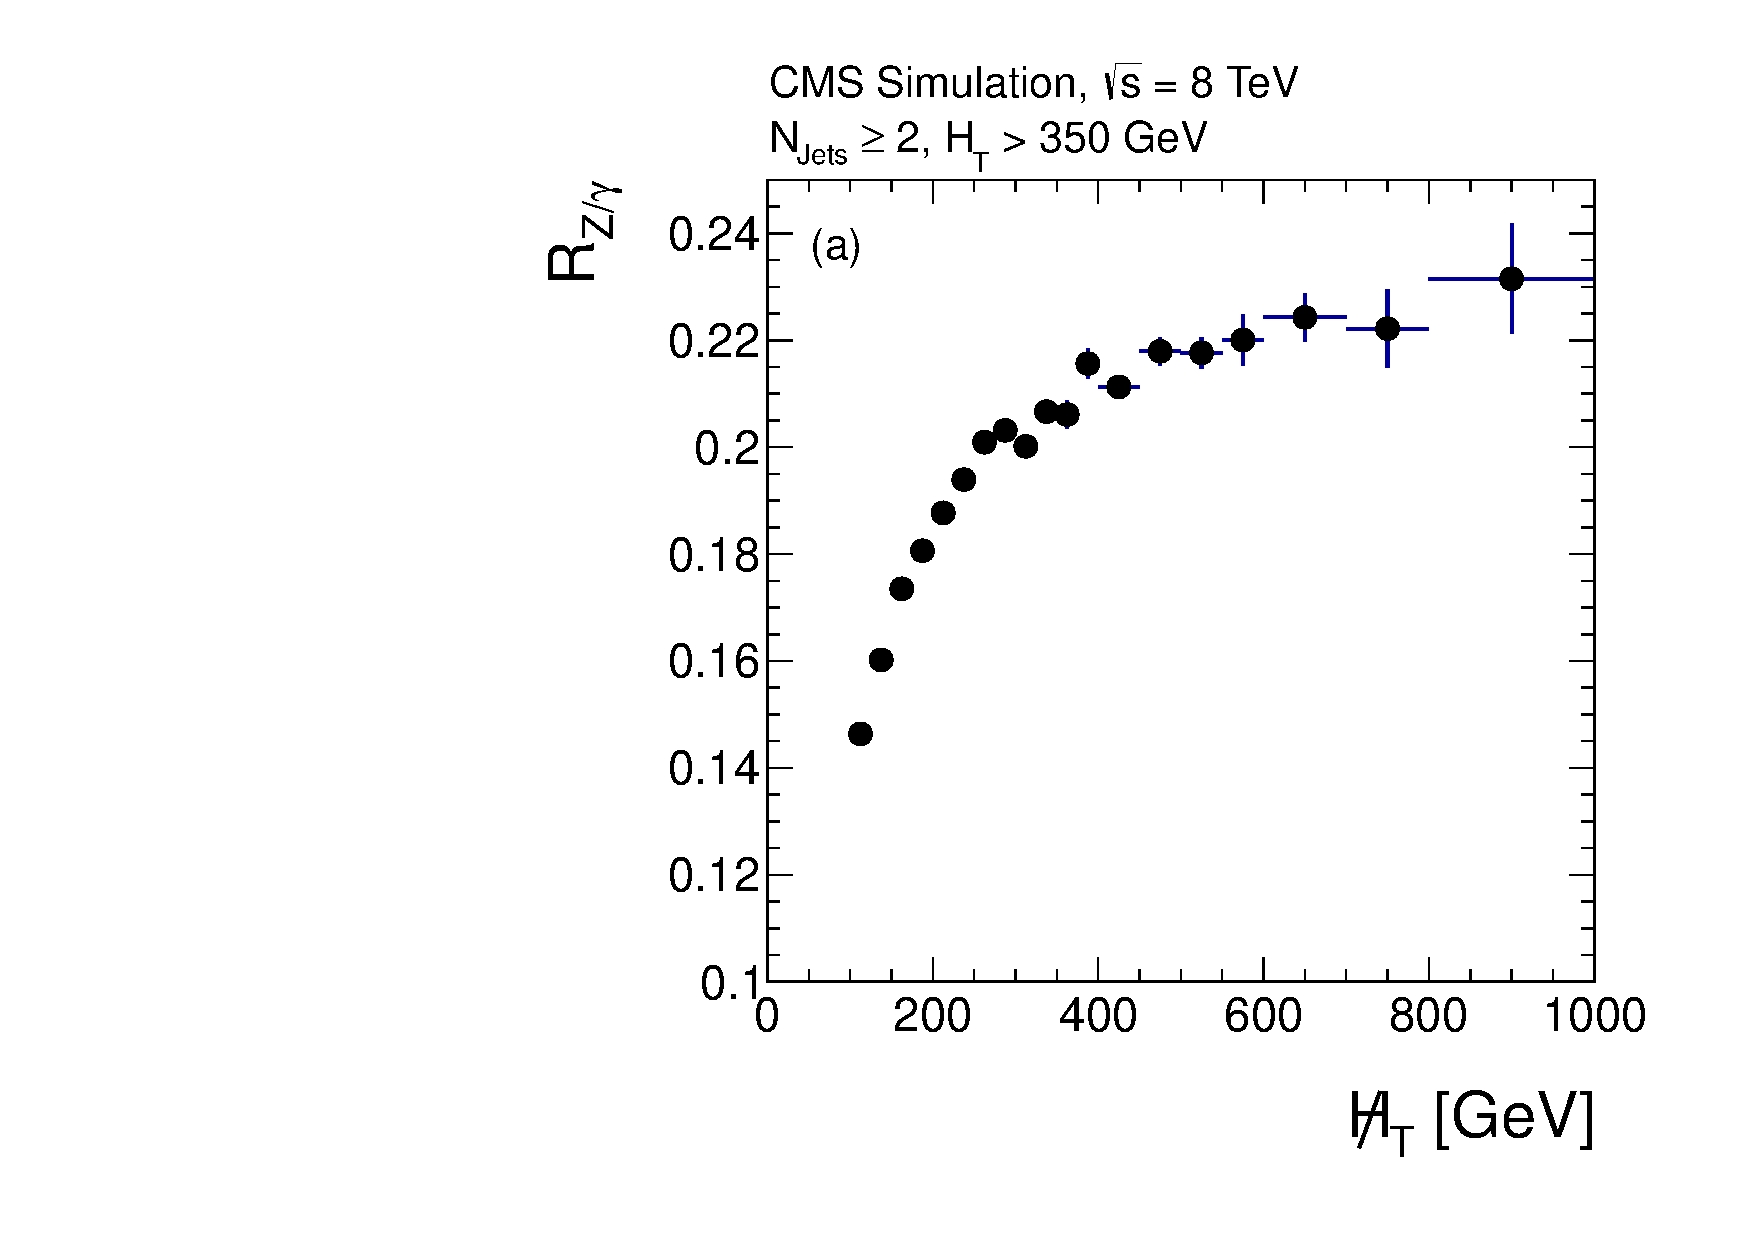
\includegraphics[width=0.4\textwidth]{figures/RA2_Zinv1.pdf} & 
                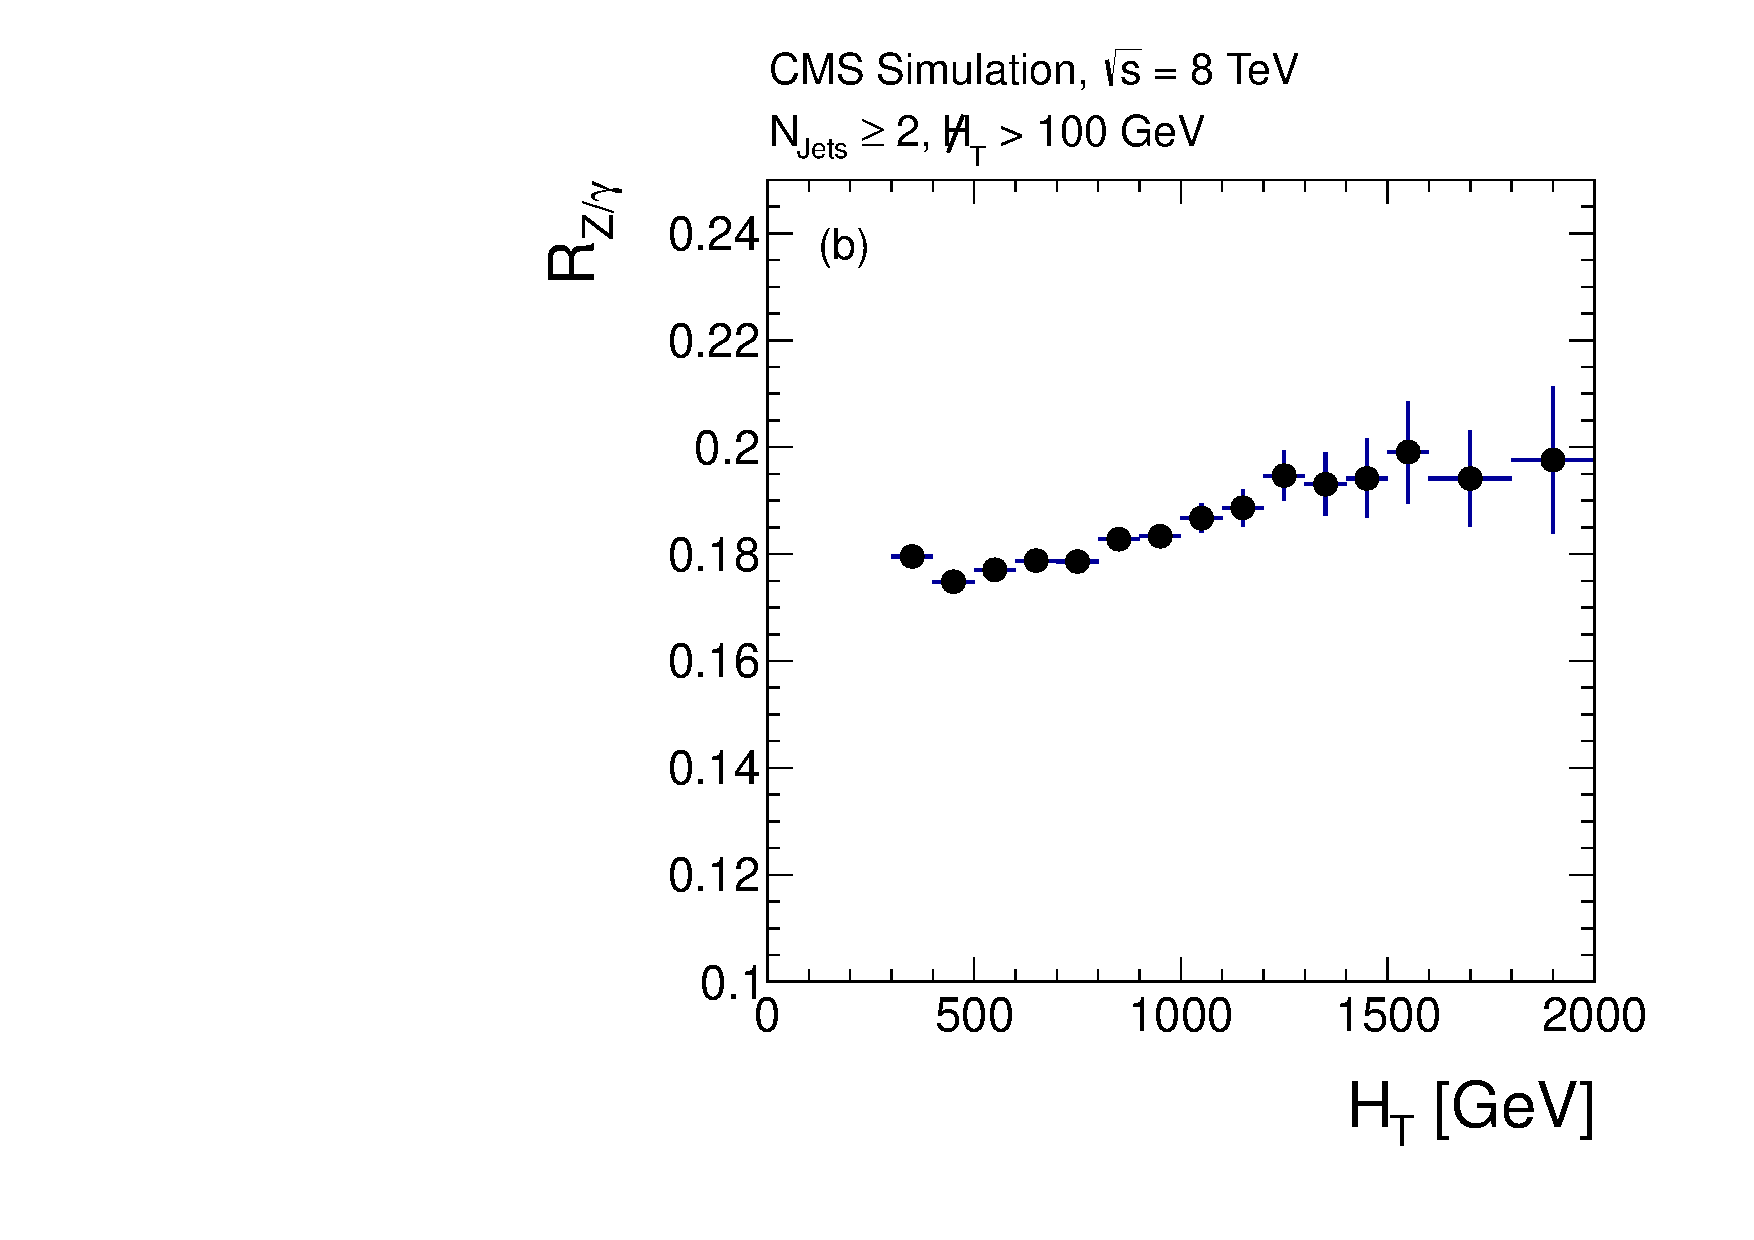
\includegraphics[width=0.4\textwidth]{figures/RA2_Zinv2.pdf} \\
                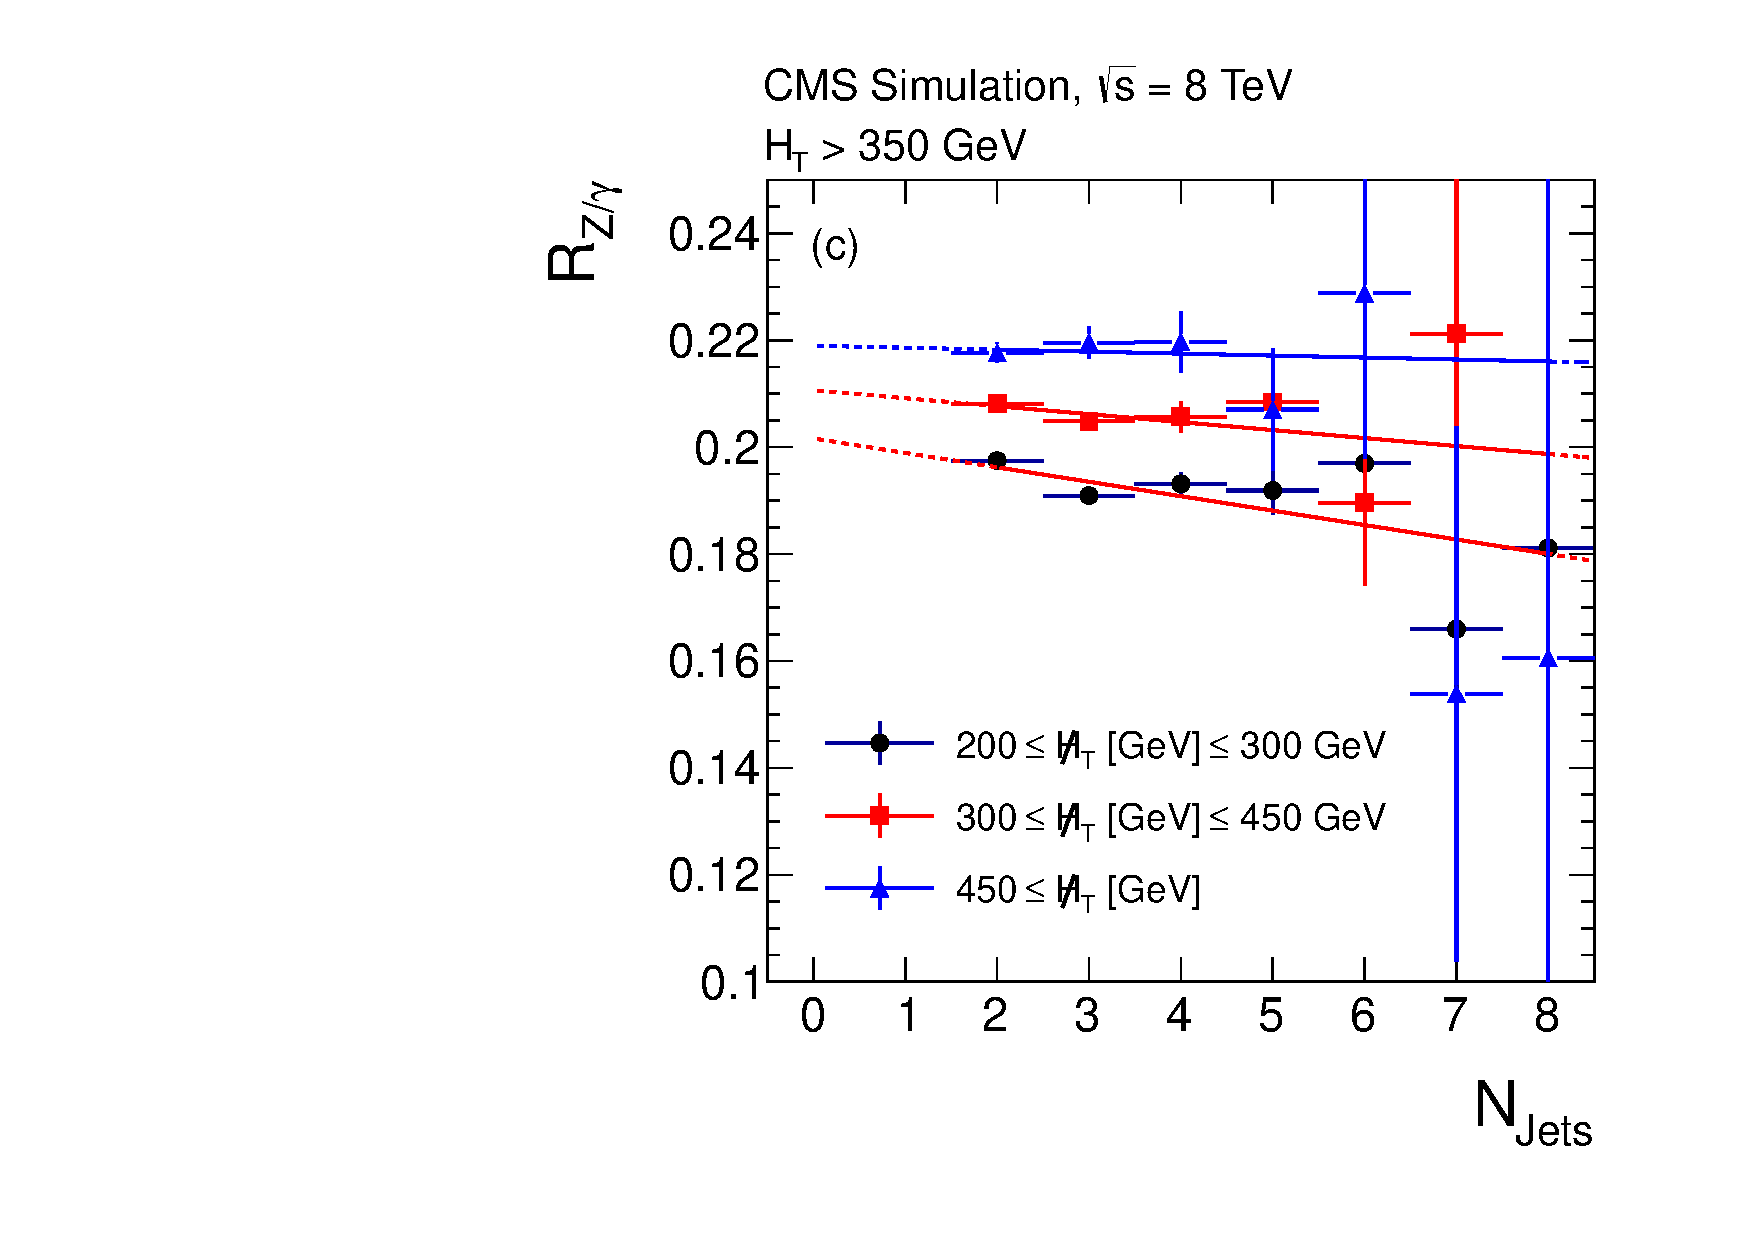
\includegraphics[width=0.4\textwidth]{figures/RA2_Zinv3.pdf} &
                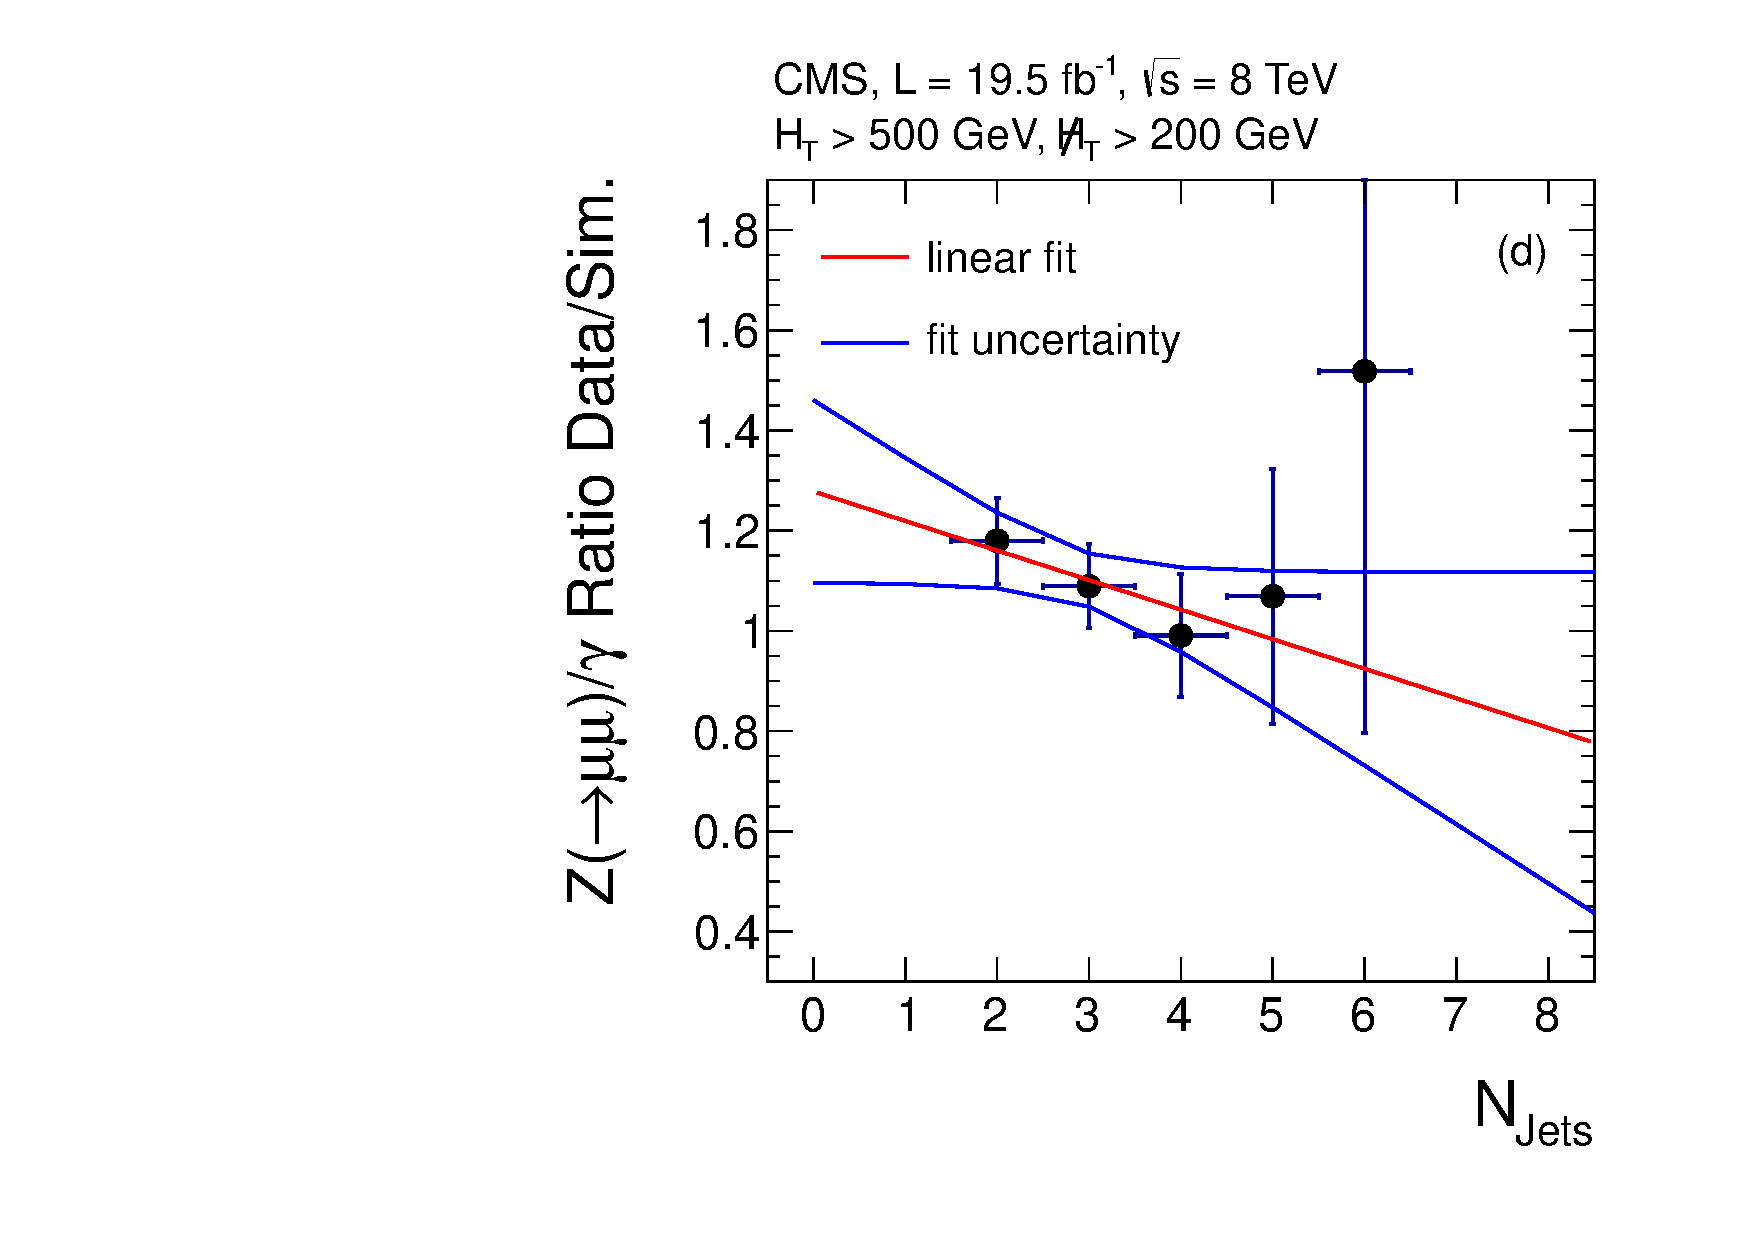
\includegraphics[width=0.4\textwidth]{figures/RA2_Zinv4.pdf}
  \end{tabular}}
  \caption{The simulated ratio $R_{Z/\gamma}$ as a function of (a) MHT, (b) HT, (c) NJets, where the values for three MHT bins are shown with linear fits, and (d) the double ratio of $R_{Z(\mu+\mu-)/\gamma}$, using events from data to those from simulation; the linear fit and its uncertainty band are overlaid. Taken from~\cite{Chatrchyan:2014lfa}.}
  \label{fig:ra2_zinv}
\end{figure}

\subsection{Hadronic $\tau$ Background}
\label{subsec:RA2_tauhad}

\begin{figure}[!h]
  \centering
\makebox[\linewidth]{
  \begin{tabular}{ccc}
                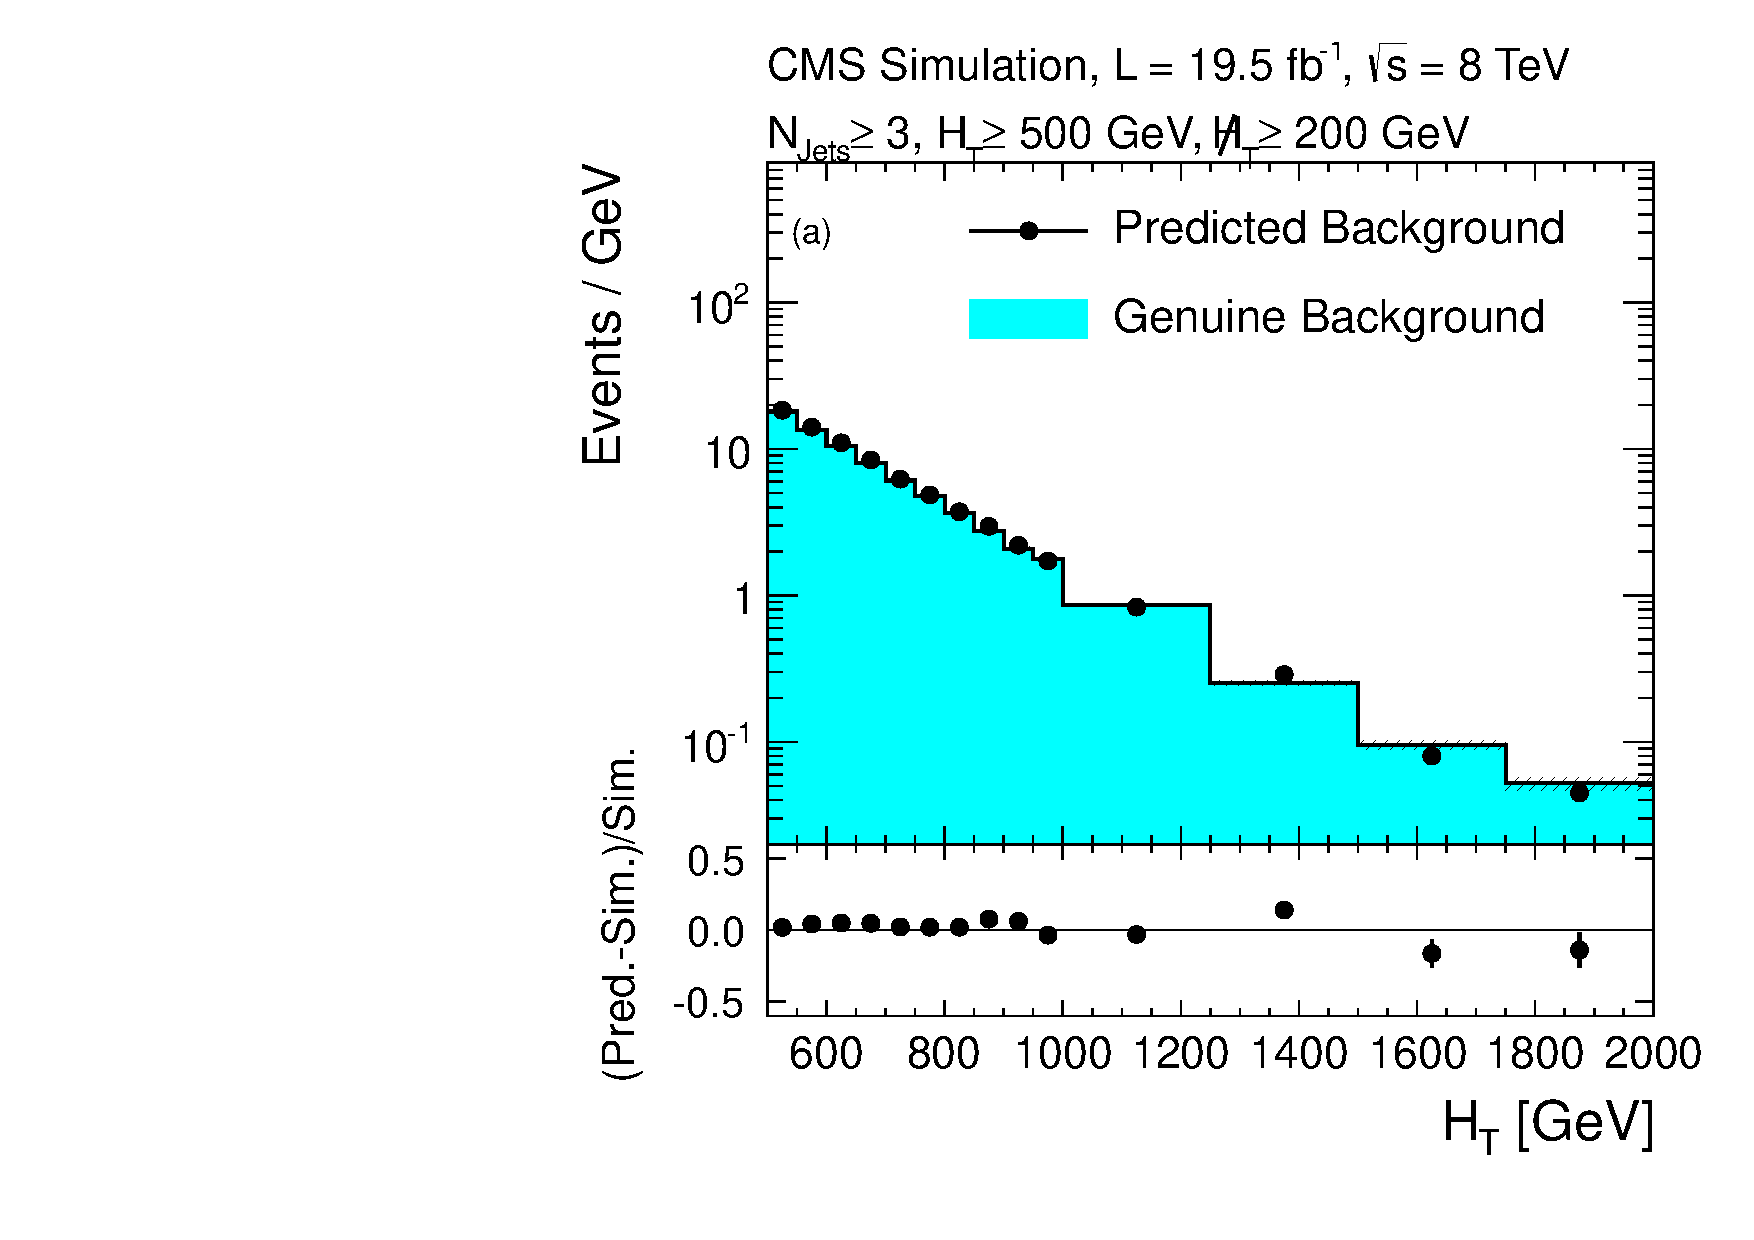
\includegraphics[width=0.4\textwidth]{figures/RA2_TauHad1.pdf} & 
                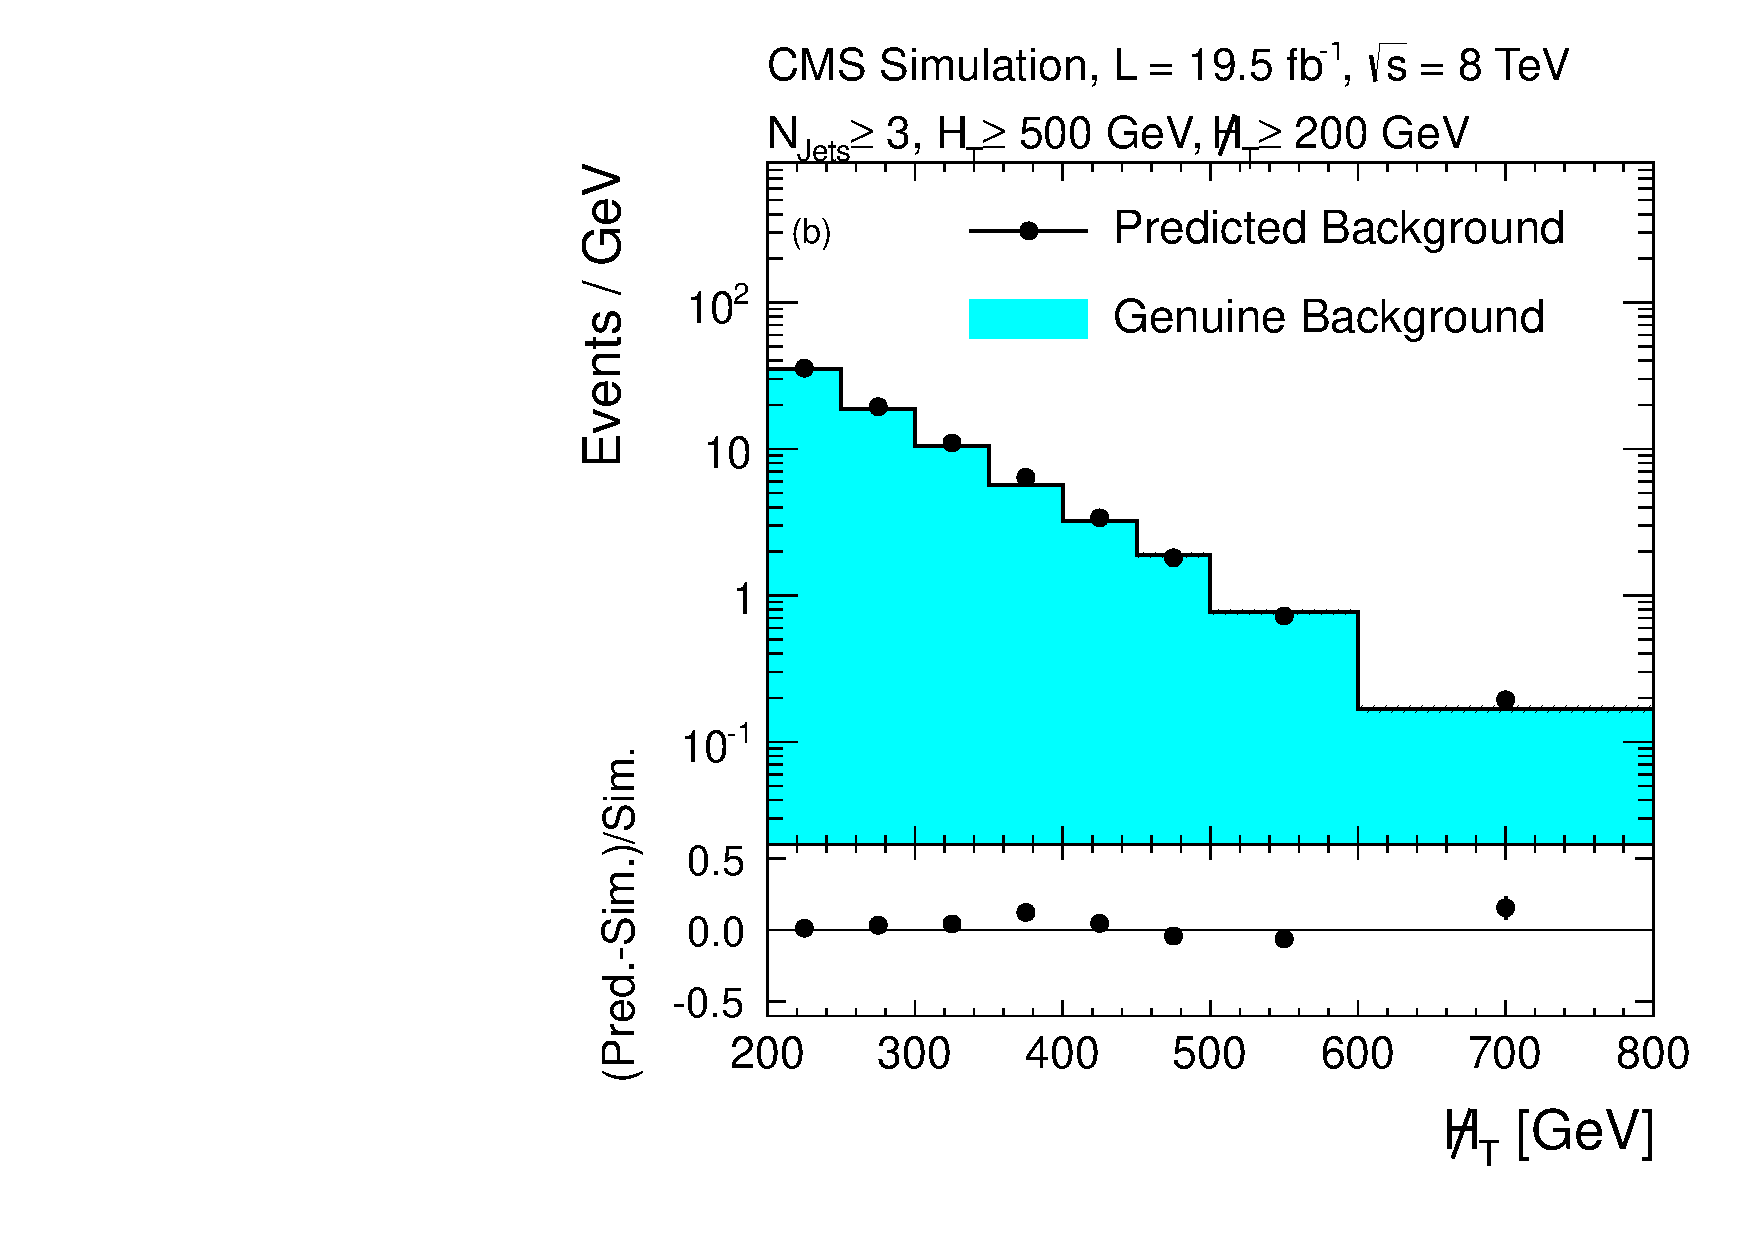
\includegraphics[width=0.4\textwidth]{figures/RA2_TauHad2.pdf} &
                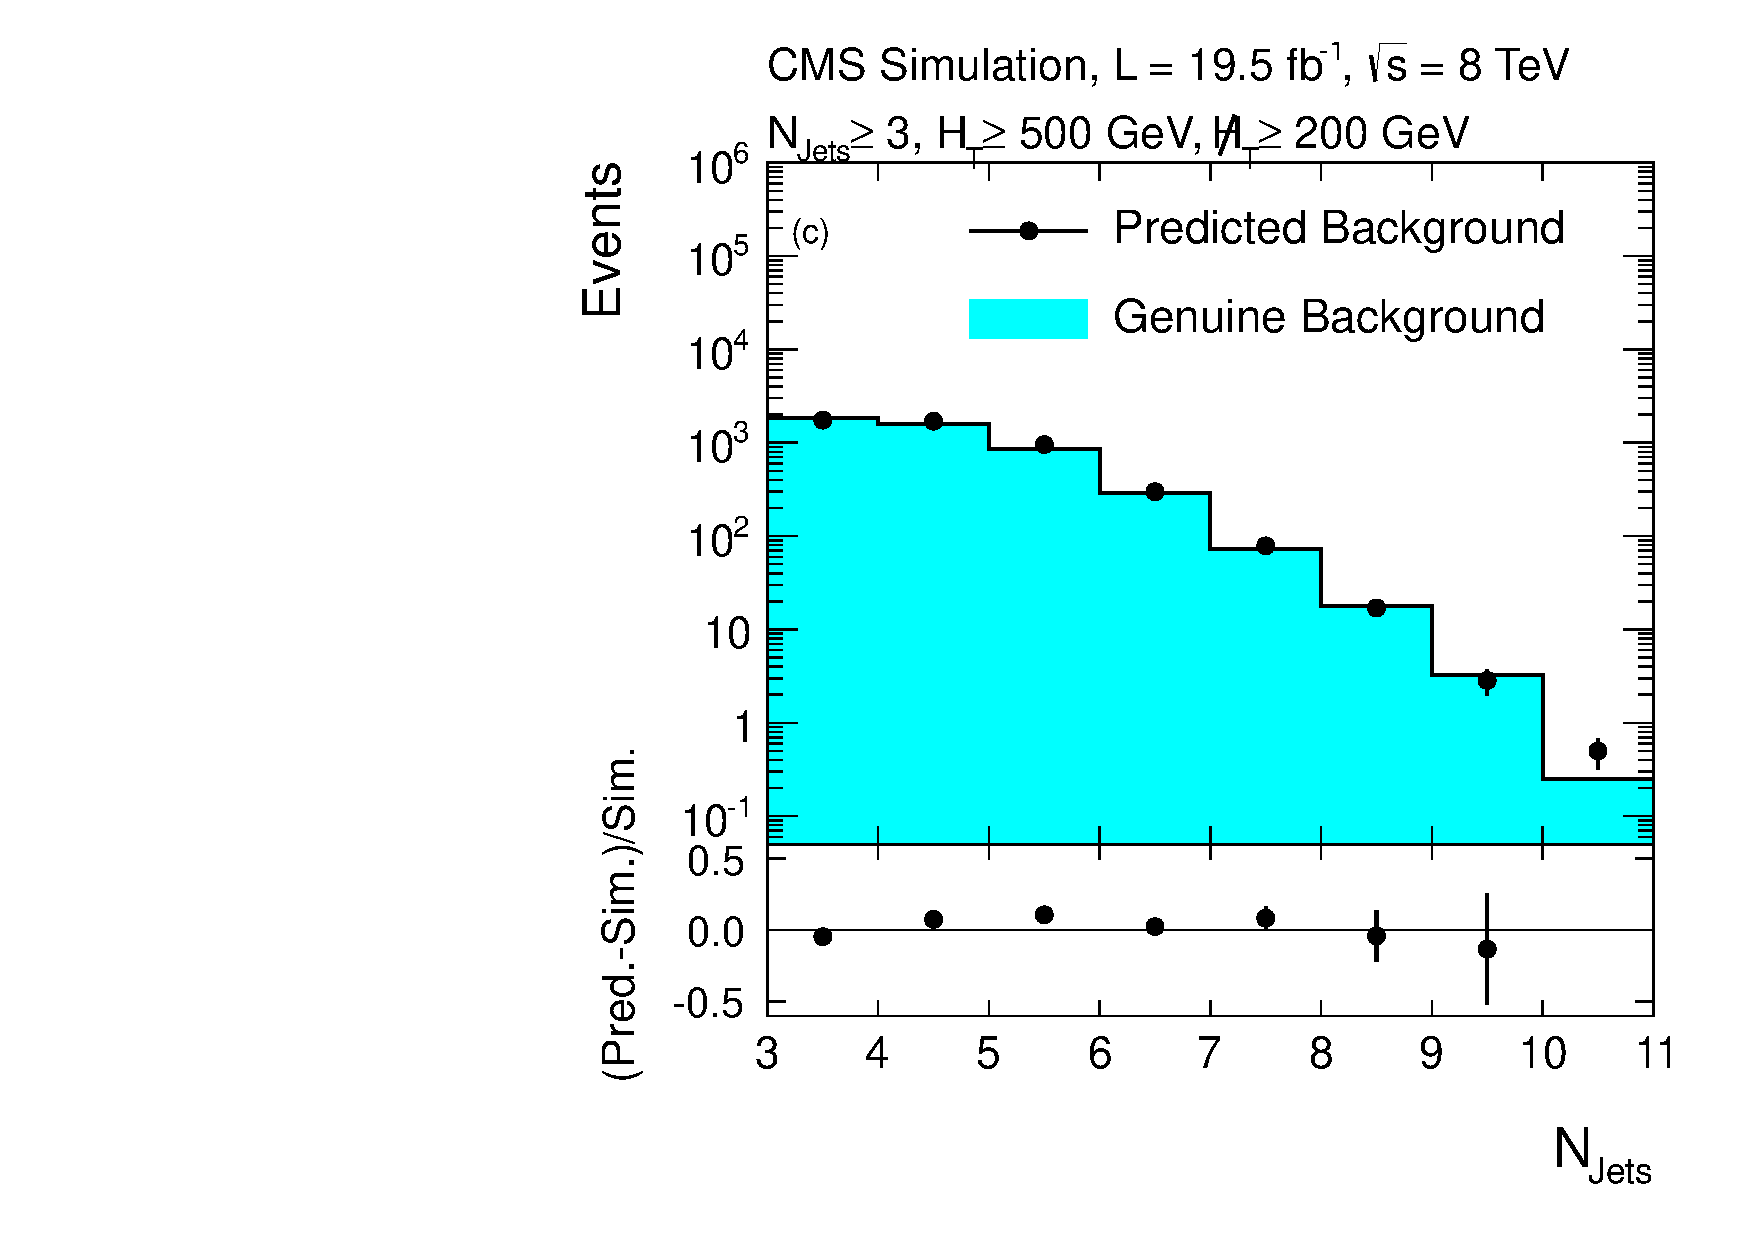
\includegraphics[width=0.4\textwidth]{figures/RA2_TauHad3.pdf}
  \end{tabular}}
  \caption{Predicted (a) HT, (b) MHT, and (c) NJets distributions found from applying the hadronic-tau background evaluation method to simulated $t\bar{t}$ and W+jets events (solid points) in comparison to the genuine $t\bar{t}$ and W+jets background from simulation (shaded curve). Only statistical uncertainties are shown. Taken from~\cite{Chatrchyan:2014lfa}.}
  \label{fig:ra2_tauhad}
\end{figure}

\subsection{Lost-Lepton Background}
\label{subsec:RA2_lostlepton}

\begin{figure}[!h]
  \centering
\makebox[\linewidth]{
  \begin{tabular}{ccc}
                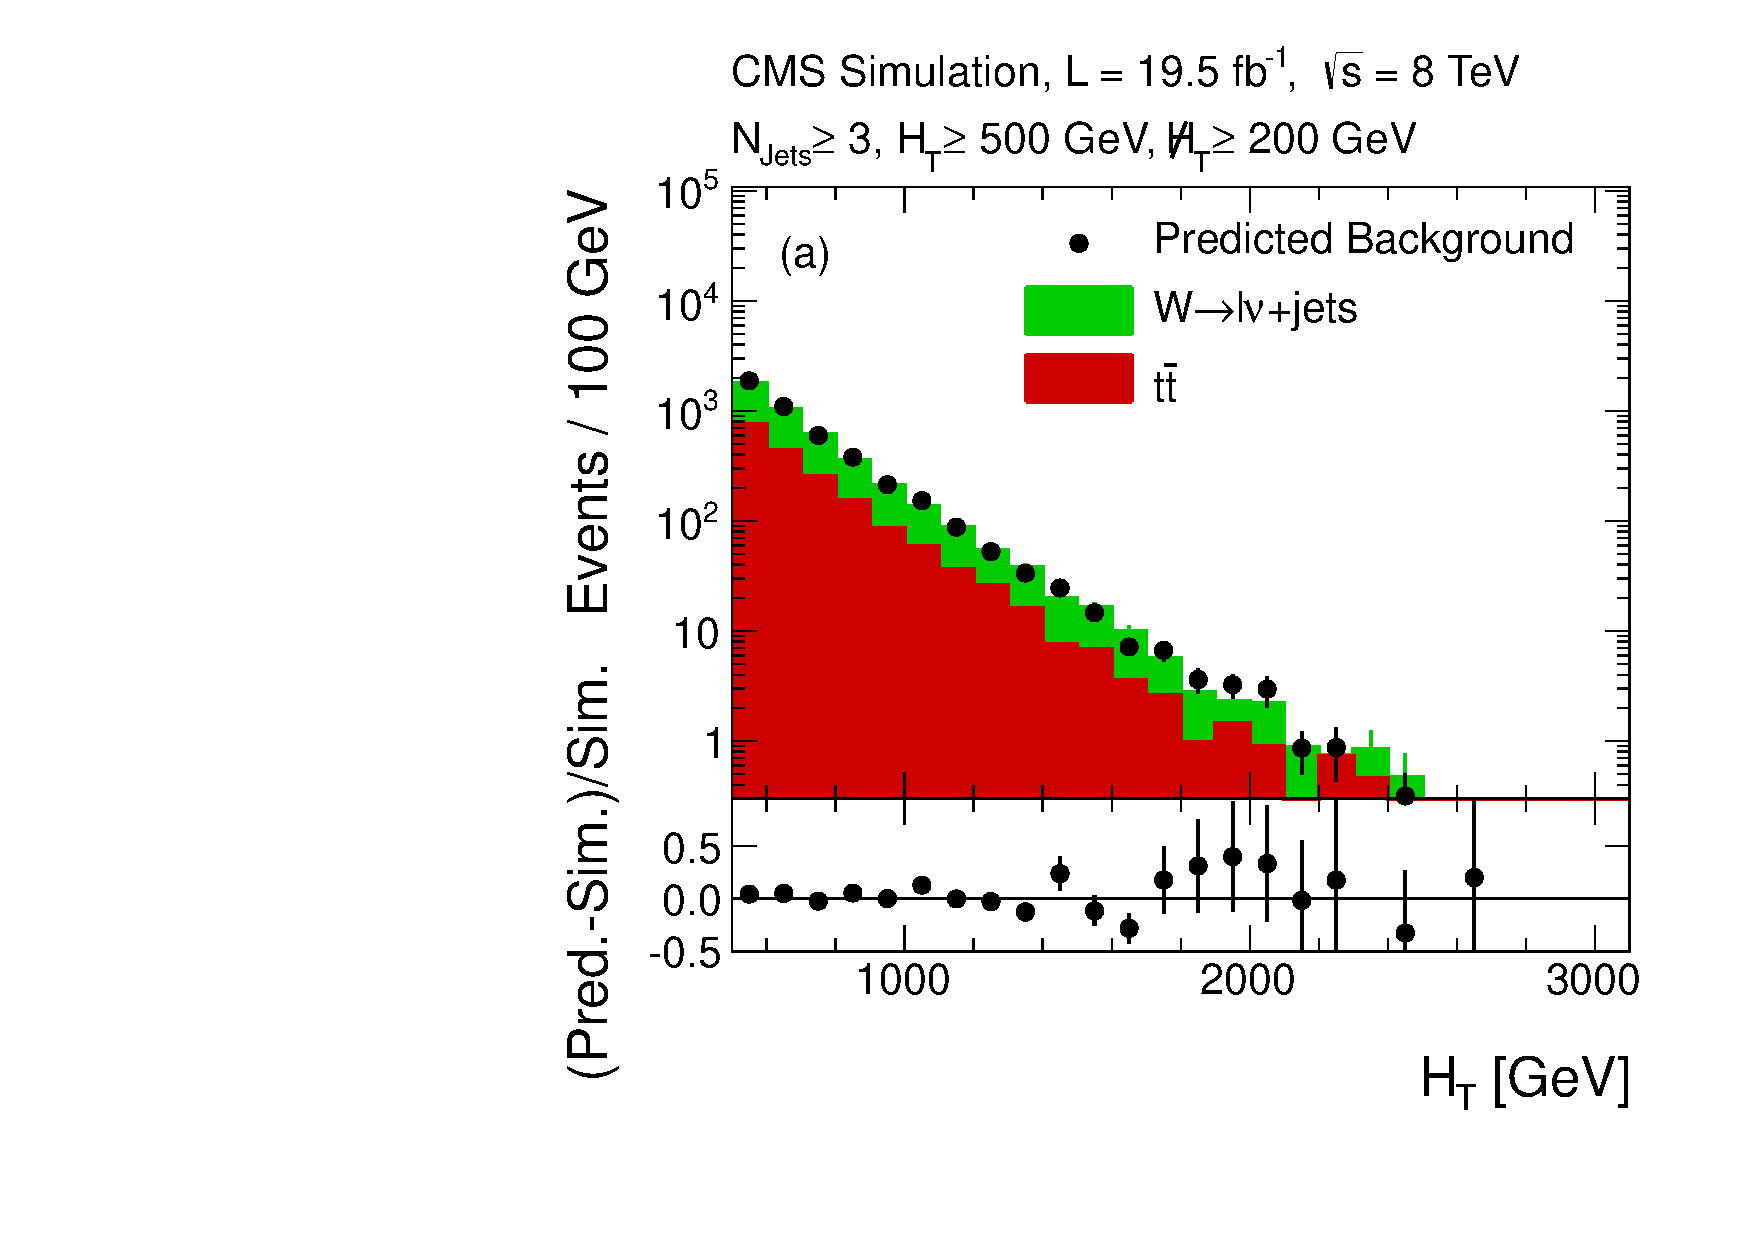
\includegraphics[width=0.4\textwidth]{figures/RA2_LL1.pdf} & 
                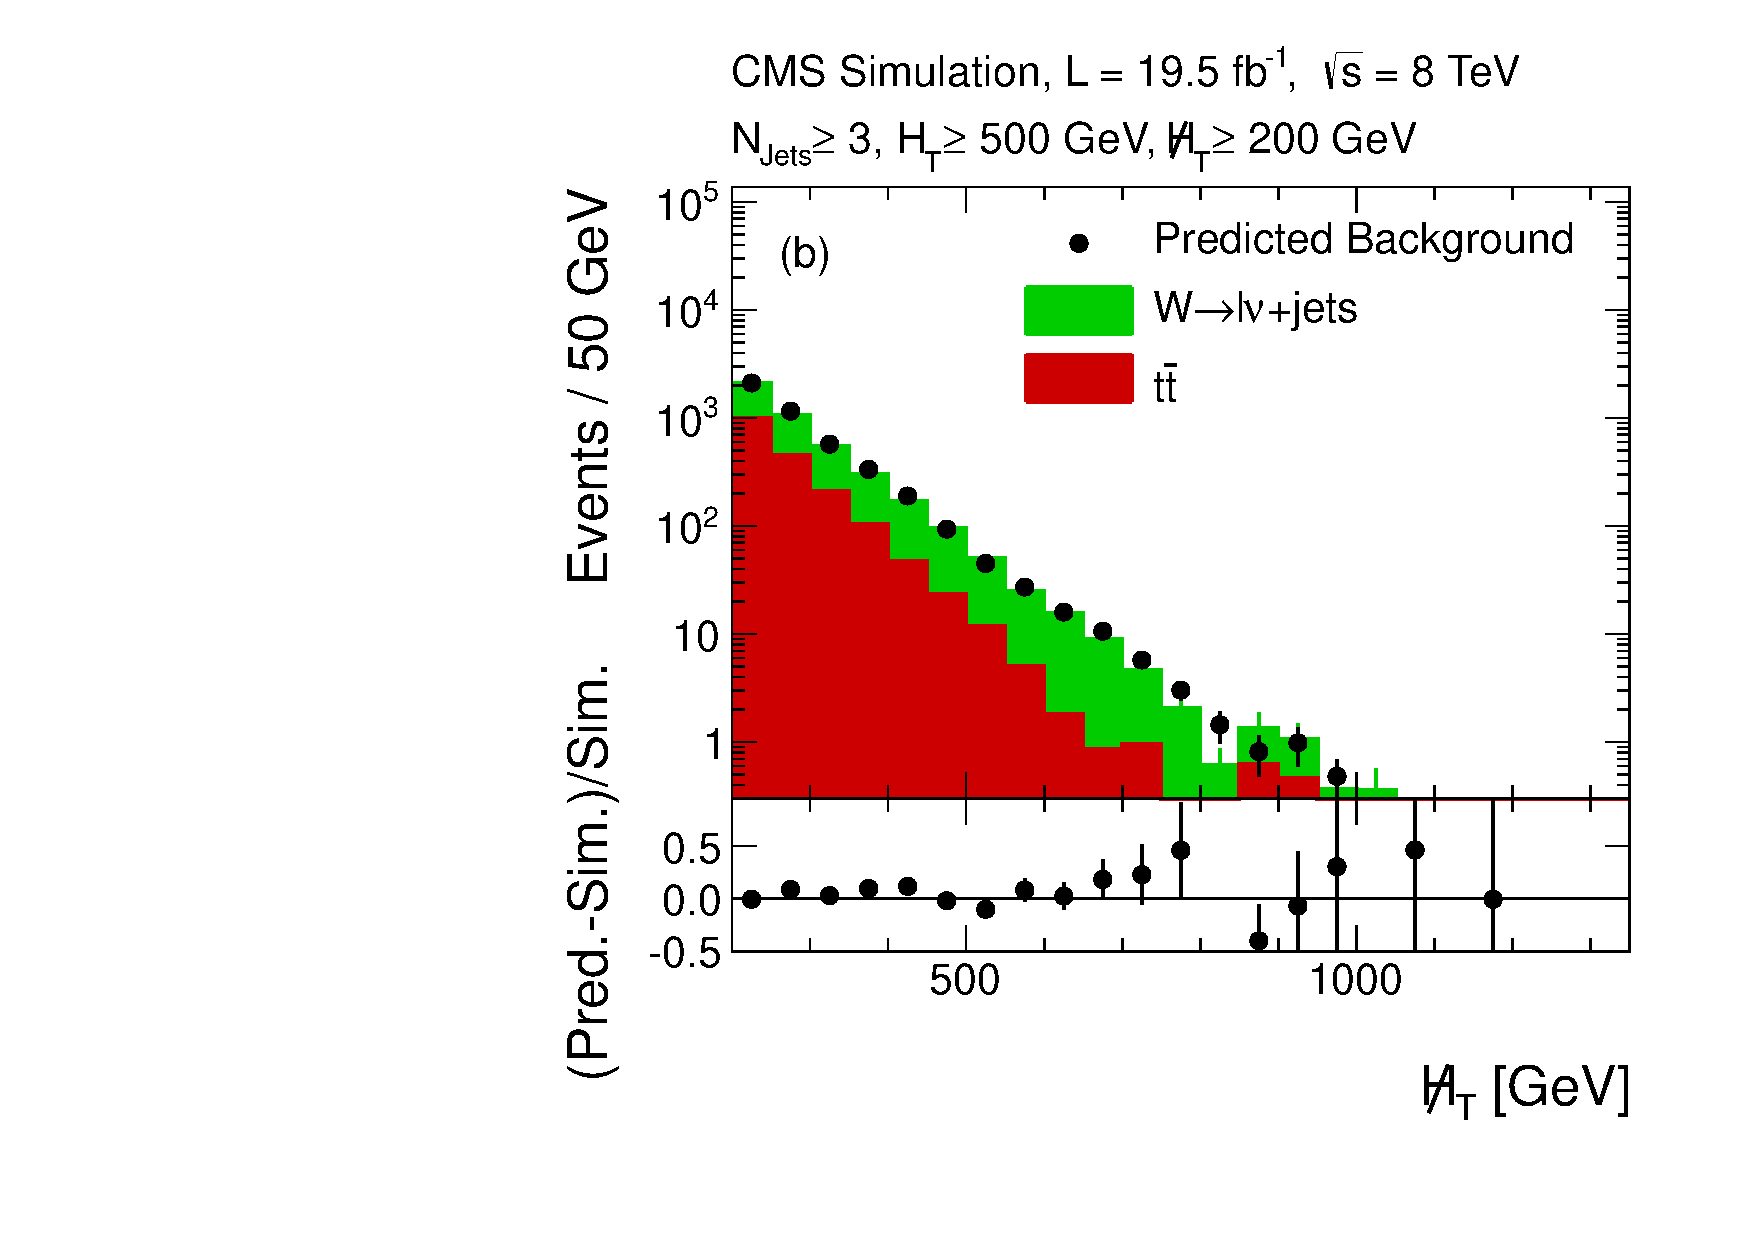
\includegraphics[width=0.4\textwidth]{figures/RA2_LL2.pdf} &
                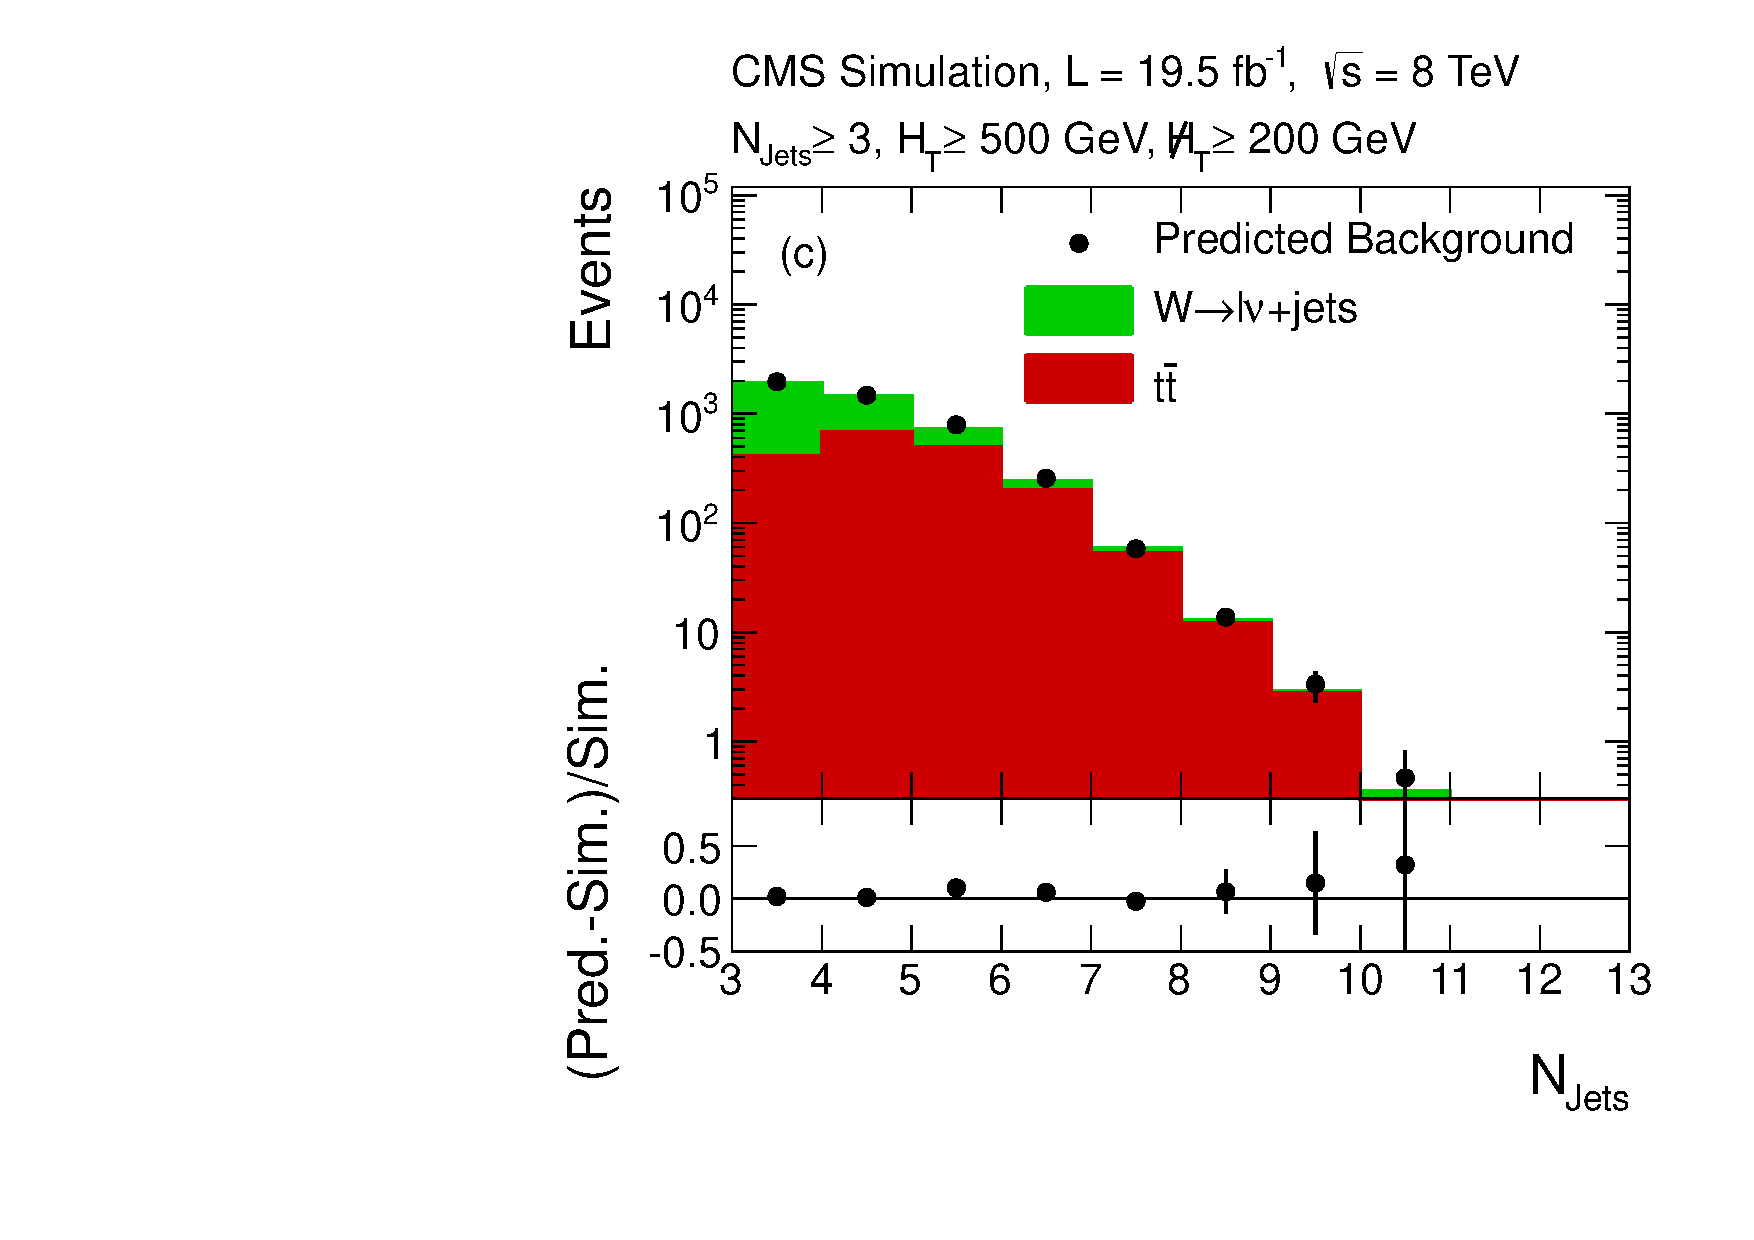
\includegraphics[width=0.4\textwidth]{figures/RA2_LL3.pdf}
  \end{tabular}}
  \caption{Predicted (a) HT, (b) MHT, and (c) NJets distributions found from applying the lost lepton background evaluation method to simulated $t\bar{t}$ and W+jets events (solid points) in comparison to the genuine $t\bar{t}$ and W+jets background from simulation (shaded curves). Only statistical uncertainties are shown. Taken from~\cite{Chatrchyan:2014lfa}.}
  \label{fig:ra2_ll}
\end{figure}

\section{Results and Interpretation}
\label{sec:RA2_results}

\subsection{Comparison to Other Measurements}
\label{subsec:RA2_comp}

\begin{figure}[!tp]
  \centering
  \begin{tabular}{c}
    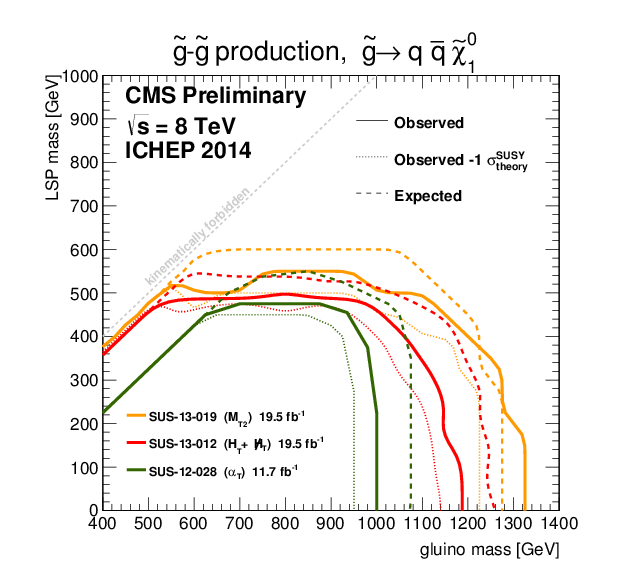
\includegraphics[width=0.9\textwidth]{figures/T1_ICHEP2014_All.png}
  \end{tabular}
  \caption{Comparison of various exclusion limits derived by different CMS analyses for the SMS T1qqqq. Taken from ... (cms susy public results).}
  \label{fig:T1_comp}
\end{figure}

\begin{figure}[!tp]
  \centering
  \begin{tabular}{c}
    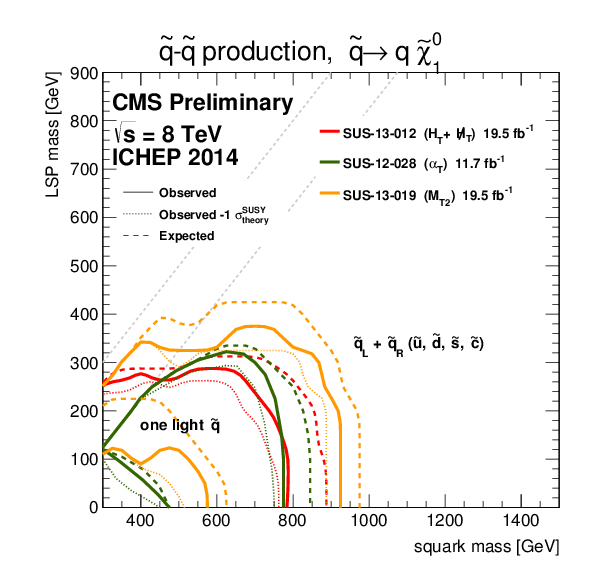
\includegraphics[width=0.9\textwidth]{figures/T2_ICHEP2014.png}
  \end{tabular}
  \caption{Comparison of various exclusion limits derived by different CMS analyses for the SMS T2qq. Taken from ... (cms susy public results).}
  \label{fig:T1_comp}
\end{figure}

\begin{figure}[!tp]
  \centering
  \begin{tabular}{c}
    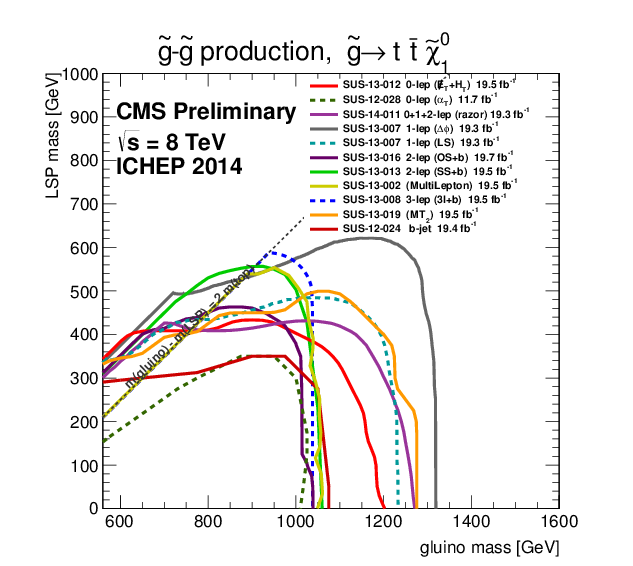
\includegraphics[width=0.9\textwidth]{figures/T1tttt_ICHEP2014_All.png}
  \end{tabular}
  \caption{Comparison of various exclusion limits derived by different CMS analyses for the SMS T1tttt. Taken from ... (cms susy public results).}
  \label{fig:T1_comp}
\end{figure}

\section{Status of natural supersymmetry after LHC Run-I}
\label{sec:susy_status}


